\chapter{Clone}
\label{ch:clone}
\ares system offers a useful feature---Clone---which reduces the repeated work of adding the precisely same items every time. Items made available for previous courses can be \textbf{imported} from those courses to the current ones. Check out the following steps to see how.

\begin{itemize}
    \item Enter Course Home and get ready:
    \begin{enumerate}
        \item From {\imp Main Menu} click on \uline{View Course}
        \item Under \textbf{Instructor Course Tools} Click on {\imp Add Reserve Items} 
    \end{enumerate}
    \item Begin to import items (see~\autoref{fig:import}):
    \begin{enumerate}
        \item Instead of selecting an item form request, select a course from the table labeled \textbf{Or would you like to import from another course?}
        \item Click on the \textbf{Import Items} link next to the course that you want to import from.
        \item On the next screen, select the items you want to import and then click on the \importbut{Import Items} button.
        \item Ares will bring you back to the \textbf{Course Details} page and confirm the import.
    \end{enumerate}
\end{itemize}

\vspace*{4ex}
\begin{figure}[h]
    \centering
    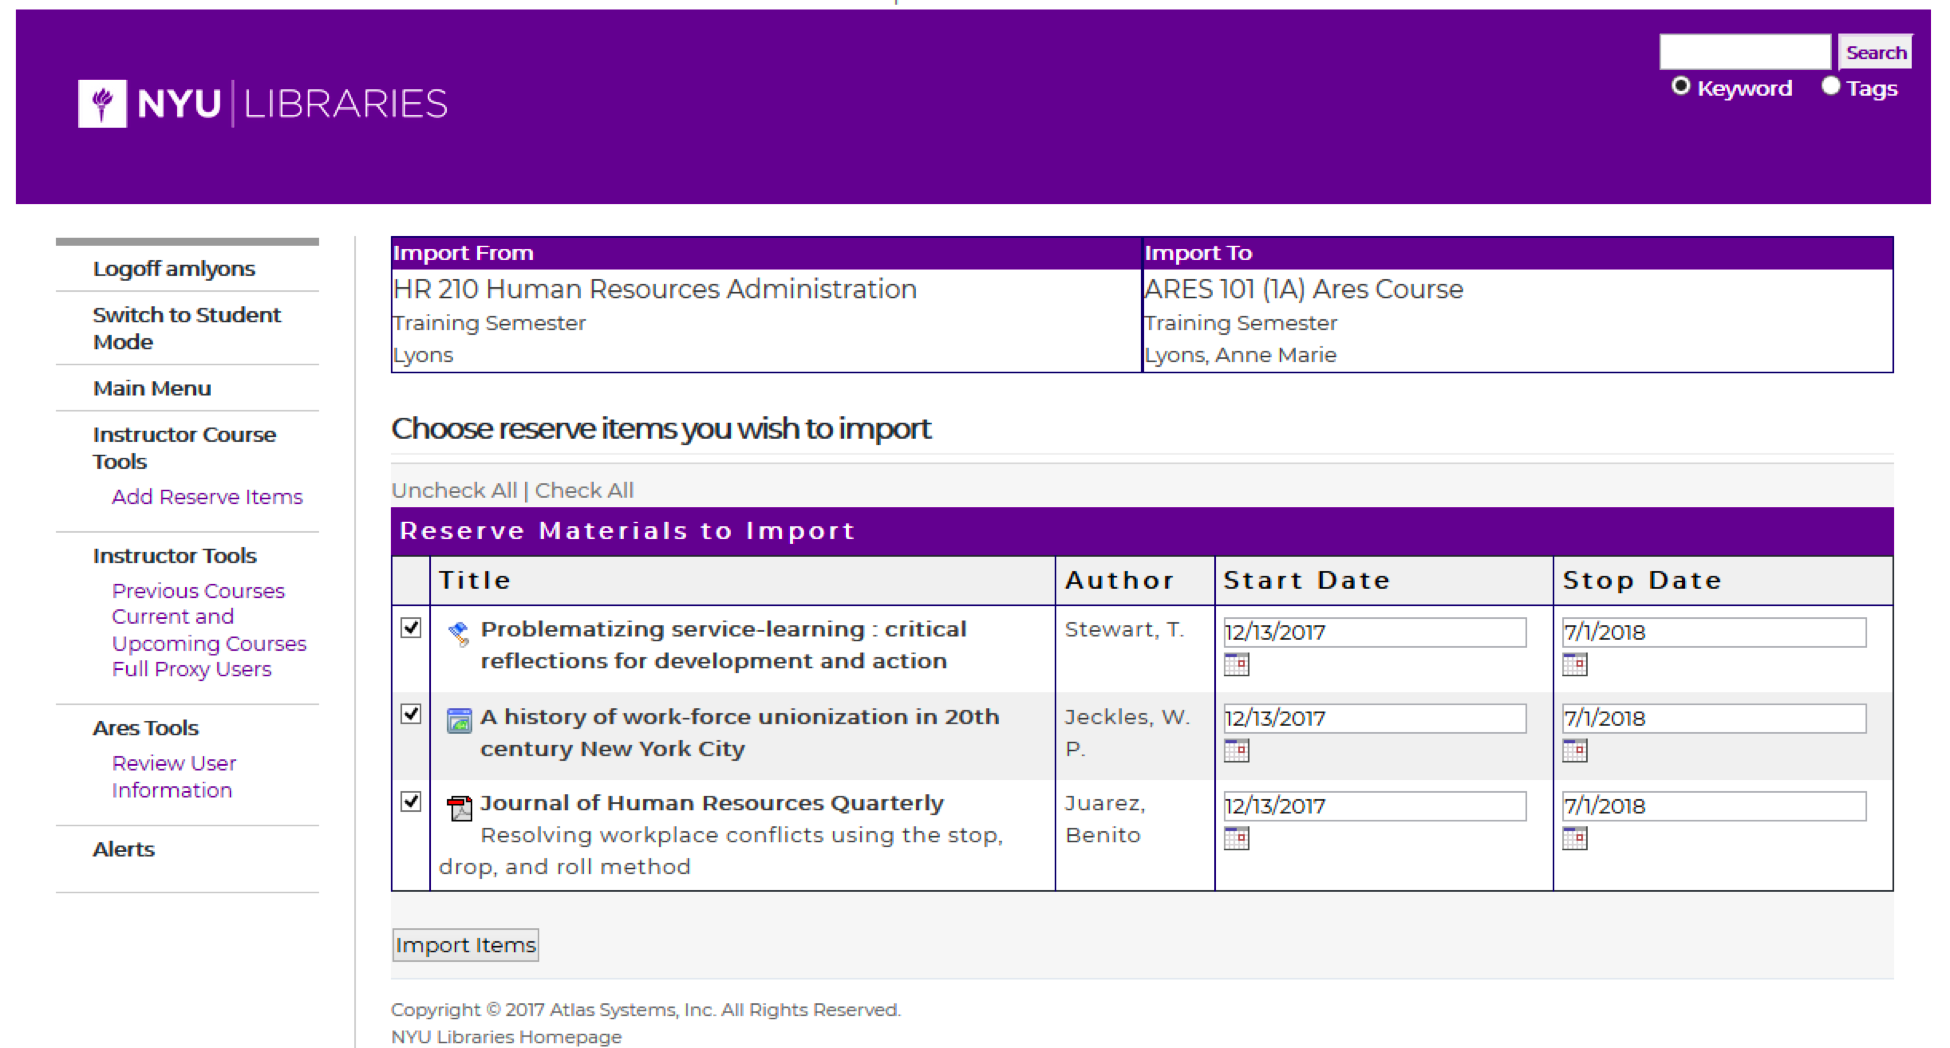
\includegraphics[width=\linewidth, height=8.5cm]{Clone}
    \caption{Import Items}
    \label{fig:import}
\end{figure}